%%%%%%%%%%%%%%%%%%%%%%% file template.tex %%%%%%%%%%%%%%%%%%%%%%%%%
%
% This is a template file for Web of Conferences Journal
%
% Copy it to a new file with a new name and use it as the basis
% for your article
%
%%%%%%%%%%%%%%%%%%%%%%%%%% EDP Science %%%%%%%%%%%%%%%%%%%%%%%%%%%%
%
%%%\documentclass[option]{webofc}
%%% "twocolumn" for typesetting an article in two columns format (default one column)
%
\documentclass{webofc}
\usepackage[varg]{txfonts}   % Web of Conferences font
\usepackage{hyperref}
%\usepackage{wrapfig}
%
% Put here some packages required or/and some personnal commands
%
%
% Indico: https://indico.cern.ch/event/773049/abstracts/106037/
% Instructions here: https://indico.cern.ch/event/773049/page/19236-proceedings
% CHEP Drive Dir: https://drive.google.com/drive/folders/1myHVCDKxmSiUk1jugDxB2lH5vc4neocQ
    % Notes document: https://docs.google.com/document/d/1wiyfZdiGGeLwcZ_j7Sq9y--xTHsVccZJLlOW5t0qGhA/edit?usp=sharing


\begin{document}
%
\title{A Lightweight Door into Non-Grid Sites}
%
% subtitle is optionnal
%
%%%\subtitle{Do you have a subtitle?\\ If so, write it here}

\author{\firstname{Jeffrey} \lastname{Dost}\inst{1}\fnsep\thanks{\email{jdost@ucsd.edu}} \and
        \firstname{Marco} \lastname{Mascheroni}\inst{1}\fnsep\thanks{\email{marco.mascheroni@cern.ch}} \and
        \firstname{Brian} \lastname{Bockelman}\inst{5} \and
        \firstname{Lincoln} \lastname{Bryant}\inst{2} \and
        \firstname{Timothy} \lastname{Cartwright}\inst{3} \and
        \firstname{Edgar} \lastname{Fajardo}\inst{1} \and        
        \firstname{Robert} \lastname{Gardner}\inst{2} \and
        \firstname{James} \lastname{Letts}\inst{1} \and
        \firstname{Brian} \lastname{Lin}\inst{3} \and        
        \firstname{M\'aty\'as} \lastname{Selmeci}\inst{3} \and
        \firstname{Igor} \lastname{Sfiligoi}\inst{1} \and
        \firstname{Judith} \lastname{Stephen}\inst{2} \and
        \firstname{Derek} \lastname{Weitzel}\inst{4} \and
        \firstname{Frank} \lastname{W\"urthwein}\inst{1} \and
        \firstname{Huijun} \lastname{Zhu}\inst{4}
}

\institute{University of California San Diego,  La Jolla, CA, USA
\and
           University of Chicago, Chicago, IL, USA
\and
           University of Wisconsin-Madison, Madison, WI, USA
\and
           University of Nebraska-Lincoln, Lincoln, NE, USA
\and
           Morgridge Institute for Research, Madison, WI, USA
          }

\abstract{%
The Open Science Grid (OSG) provides a common service for resource providers and scientific institutions, and supports sciences such as High Energy Physics, Structural Biology, and other community sciences. As scientific frontiers expand, so does the need for resources to analyze new data. For example, High Energy Physics experiments such as the LHC experiments foresee an exponential growth in the amount of data collected, which comes with corresponding growth in the need for computing resources. Allowing resource providers an easy way to share their resources is paramount to ensure the grow of resources available to scientists.

In this context, the OSG Hosted CE initiative provides site administrator a way to reduce the effort needed to install and maintain a Compute Element (CE), and represents a solution for sites who do not have the effort and expertise to run their own Grid middleware. An HTCondor Compute Element is installed on a remote VM at UChicago for each site that joins the Hosted CE initiative. The hardware/software stack is maintained by OSG Operations staff in a homogeneus and automated way, providing a reduction in the overall operational effort needed to maintain the CEs: one single organization does it in an uniform way, instead of each single resource provider doing it in their own way. Currently, more than 20 institutions joined the Hosted CE initiative. This contribution discusses the technical details behind a Hosted CE installation, highlighting key strengths and common pitfalls, and outlining future plans to further reduce operational experience.
}
%
\maketitle
%
\section{Introduction}
\label{intro}
Grid computing\cite{foster2003grid} has been the technology of choice to address the distributed computational needs of many scientific fields like High Energy Physics, Structural Biology, and other science communities. Exponential growth in the amount of data collected by those sciences comes with corresponding growth in the need for computing resources.

The Open Science Grid\cite{OSG} (OSG) is a national, distributed computing partnership for data-intensive research that facilitates access to distributed high throughput computing for different research communities in the US. The resources accessible through the OSG are contributed by the community, organized by the OSG, and governed by the OSG consortium. 

Allowing resource providers (sites) an easy way to share their resources is paramount to ensure that the growth of resources is available to scientists. The Hosted CE initiative by the OSG provides the site administrator a way to reduce the effort needed to install and maintain a Compute Element (CE), the Grid portal to a compute cluster, facilitating the process of sharing resources between the scientific communities served by OSG.

\section{Traditional CEs vs Hosted CEs}
\label{ces}
 A key component of the Grid infrastructure is the Compute Element (CE), a set of services that provides access to a local resource management system. Sometimes, an institution has a batch-based cluster which is served by their chosen local resource management system (Slurm, PBS, HTCondor, SGE, etc.), and it wants to share those resources with the rest of the world. In order to start receiving Grid jobs from the scientists belonging to OSG organization, an administrator belonging to the institution normally has to deploy and operate their own compute element on locally provisioned servers.


\begin{figure}[ht]
\centering
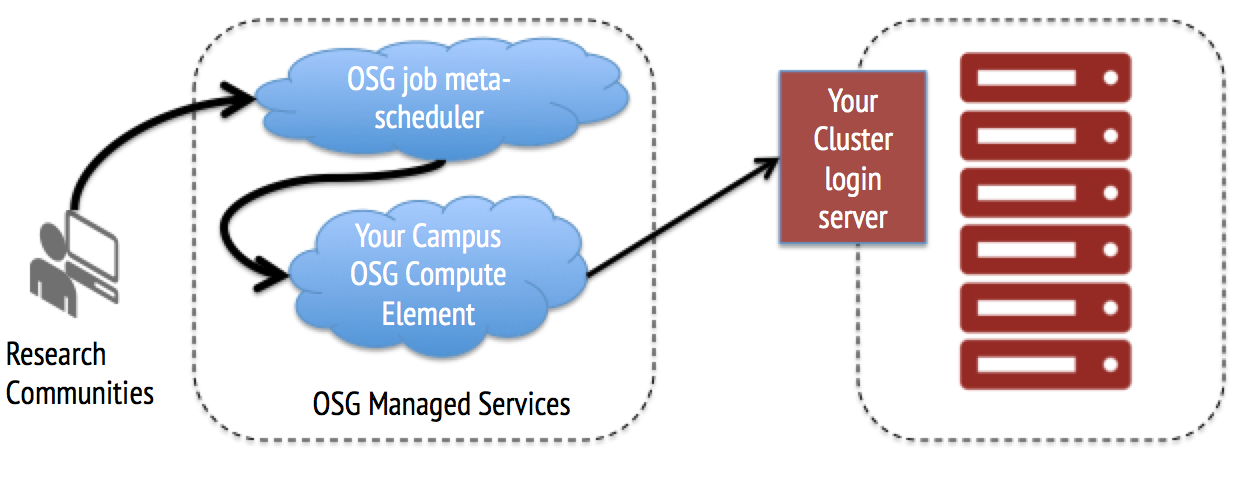
\includegraphics[width=1.0\textwidth]{images/OSGChart.png}
\caption{Interaction between different OSG services and site cluster}
\label{fig-OSG}
\end{figure}


The Hosted CE initiative addresses this issue and aims at removing the entry barrier for institutions that want to join the OSG, but lack expertise on administration of Grid system. In fact, the OSG offers the possibility to install and run and maintain all the software and the hardware needed to run a CE, offloading the complexity and responsibility of maintenance from the site administrator to grid experts (see Figure \ref{fig-OSG}). The site must simply provide an SSH login to their cluster head node. This login is then used to send jobs by an external Compute Element which is maintained by the OSG (\textbf{the Hosted CE}) on a virtual machine. From their point of view the Hosted CE users are like any other user login. This remarkably simplifies the amount of effort required to join the OSG because site administrators do not have to install and maintain any software beyond what they are already running (i.e. their local resource management system). All the institution has to do is to fill in a form\cite{HostedCE} to provide detailed contact and cluster information and satisfy some simple requirements as discussed in Subsection \ref{requirements}.


%Maybe later say that:
%special generic names, osg01, osg02, ..., osg20 that map to different VOs.

%This probably belongs to the next section
%Then OSG will contact you and ask you to grant access to a specific SSH key to your campus cluster head node. OSG will host and operate on your behalf a VM that runs the HTCondor-CE software! Also, WN client, managements of CA certs and CRL is automatically handled and nothing needs to be installed on the WN for the simplest use case (OSG jobs).

% Cite https://opensciencegrid.org/docs/compute-element/hosted-ce/

\subsection{Site Requirements}
\label{requirements}
In order to be eligible and be able to apply for a Hosted CE, the existing compute cluster needs to use a supported batch system, and it needs to run on a supported operating system. Supported batch systems are: HTCondor, LSF, PBS / TORQUE, SGE, and Slurm, while supported operating systems are Red Hat Enterprise 6 and 7 and compatible platforms (for 64-bit Intel architectures). Outbound network connectivity from the worker nodes is also required to access a list of services and hosts. Worker nodes connection can be behind a NAT (Network Address Translation). The list of services/hosts that worker nodes need to connect to includes: pilot/workload management systems, to download the scripts that are executed on the worker nodes, the HTCondor Collector and Schedulers\cite{HTCondor}, required to start receiving users' payload jobs, and optionally other services like XRootD cache servers\cite{AAA}, Squid proxies\cite{frontier}, CVMFS\cite{CVMFS} etc. Temporary scratch disk space on each worker node needs to be available. The OSG Worker Node Client needs to be distributed to the worker nodes. This is handled by the OSG staff, but if an HTCondor batch system is used, a shared file system between the cluster head node and the worker nodes is also necessary. Alternatively, the site administrator can install the Worker Node Client on the worker nodes either via RPM or tarball distribution, if they prefer to maintain it themselves. Finally, a set of Unix accounts need to be configured on the site cluster's head node, and they need to be accessible via an SSH key. The Hosted CE will use this account to automatically submit jobs through BOSCO\cite{Weitzel2014}, so these accounts must also have permissions to submit jobs to the batch system.

The following section focuses on the details required to operate the Hosted CEs from the OSG perspective. The details are hidden from the site by design, to simplify the sharing of resources on the OSG.

\section{Operating the Hosted CEs}
\label{operations}
The operation of the Hosted CEs is split into two categories: routine operations, which includes installation and configuration of new CEs, and support, which consists of monitoring for and fixing issues when things go wrong.

\subsection{Routine Operations}
\label{routine}

Routine operations consists of all activities relating to managing the software services on the Hosted CE. This includes the initial installation of the software, and proper configuration tailored to the needs of the site. The installation is unique in that some software needs to be installed on the dedicated host owned by OSG, but also other scripts and configuration files need to be staged into the non-root user home directory on the head node of the remote cluster owned by the site. All of this is managed through SSH. Care must be taken if customizations to the scripts and configurations on the head node must be modified. Software updates can inadvertently wipe changes made on the remote side. In addition, as discussed in Section \ref{requirements}, the OSG administrators provide worker node software, which includes the bundle for Public Key Infrastructure \cite{foster1998security} (PKI) Certificate Authority (CA) certificates, and scripts to keep Certificate Revocation Lists (CRLs) up to date. These are needed for pilot authentication. The Worker Node Client software is usually managed on a shared file system internal to the site and accessible from the head node user. It is then exported on all of the worker nodes in the cluster. If the remote configuration is altered, user jobs will not be able to function properly at the site.

Given the fragile nature of the customizations to the software on the remote side, that can inadvertently be wiped by software updates on the CE, the OSG Software team has worked with the Operations team and produced tools for better maintenance automation. The package containing those tools is called \emph{update-all-remote-wn-clients}. Rather than customizing the remote scripts and files in place, all modifications are stored in a single private Git repository for all CEs. The repository is then cloned onto each Hosted CE, and the update-all-remote-wn-clients scripts are run from the CE to copy the relevant files to the remote side, as well as install the Worker Node Client and CA certificates. Some other scripts are run initially on a fresh install, and also whenever changes are made. The update-all-remote-wn-clients that manages the Worker Node Client, CRLs, and customizations is run periodically every 12 hours to ensure that everything is always up to date. Having the repository has proven invaluable. If anything goes wrong on the remote side, all of the configuration is recoverable by simply re-running the install scripts.

\begin{figure}[ht]
\centering
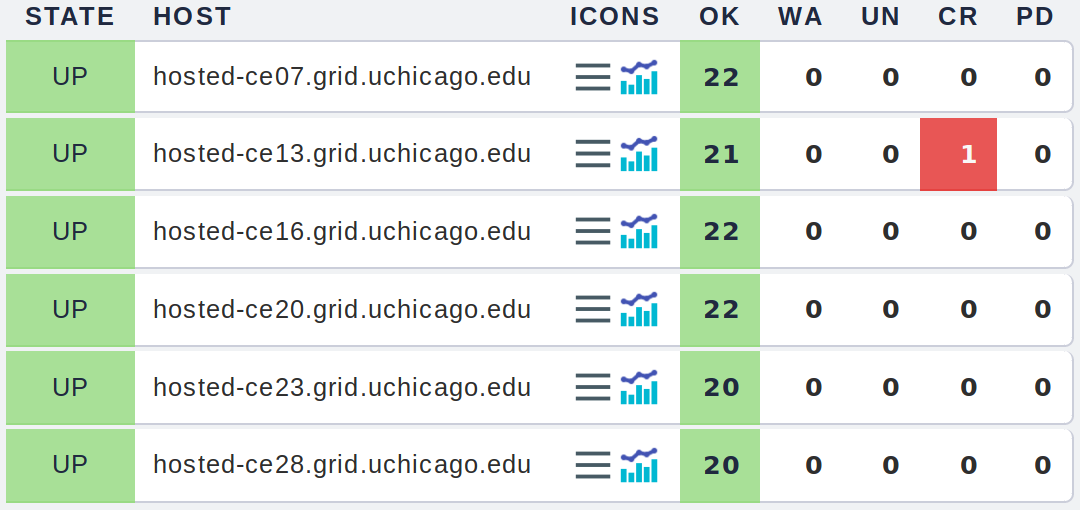
\includegraphics[width=1.0\textwidth]{images/check_mk.png}
\caption{The Check\_MK tool}
\label{fig-check_mk}
\end{figure}

\subsection{Support}
\label{support}
The support portion of Hosted CE operations consists of detecting when there are problems at any part of the infrastructure for a given Hosted CE, determining the source of the problem, and ultimately providing the solution. Operational experience has shown there are three categories of things that can disrupt the service:
\begin{enumerate}
    \item Issues encountered on the Hosted CE node
    \item Issues encountered on the site batch system
    \item Planned maintenance on the site batch system
\end{enumerate}

Some examples of issues in Category 1 include expiring host certificates, DNS resolution issues, and firewall problems. These are all things OSG operators need to be aware of, and have the access to fix directly. Examples of issues in Category 2 are the head node going down, disk issues on the shared file system, and SSH failures due to network issues between CE and head node. In order to handle Category 2 problems, the site administrator typically needs to take action since the OSG operators do not have root access on the head node. In this case, the OSG operator must open a support ticket with the site to report the issue, and allow the site administrator to resolve it on their end. Finally, Category 3 are intentional temporary disruptions of service on the site batch side to handle routine maintenance. While disruptions of this type do not indicate a problem, it is important for the site administrator to communicate to the Hosted CE operators in advance that the outage will happen, otherwise it could be confused with an unplanned Category 2 issue.

Tools to automatically detect issues with CE have been developed on top of Check\_MK \cite{CheckMK}, a popular service monitoring tool for distributed systems (see Figure \ref{fig-check_mk}). The Check\_MK monitoring allows OSG staff to monitor the health of the Hosted CEs, receive alerts when things go wrong, and generate monthly availability email reports to be sent to OSG management. The Check\_MK monitoring has helped the OSG Operations team stay on top of debugging and fixing issues in a timely manner. However, the system is still in its infancy, and there is room for improvement. While the current Check\_MK tests are great at alerting on service disruptions, the system does not yet have the ability to automatically flag which category they fall under. Having the ability to categorize the disruption type from the monitoring would reduce the manual overhead currently needed to determine it, which is crucial in informing the subsequent actions required to resolve the issue.

%OSG staff is in charge of communications with site administrators in case of problems.

%Operations uses Checkmk based tools to:
%\begin{itemize}
%    \item Monitor health of the CEs
%    \item Receive alerts when things go wrong
%    \item Generate monthly availability email reports
%\end{itemize}

\section{Future Plans}
\label{future}

% JD covered in section 3, need to talk about SLATE here instead
%Joint effort between the OSG Software and Operations teams has improved the management of the Hosted CEs by implementing tools to:
%\begin{itemize}
%    \item Track Hosted CE configuration in version control
%    \item Manage site-specific configuration and hot fixes
%    \item Automate worker node data and software updates
%\end{itemize}

The OSG Software and Operations teams have been working together to provide a solution based on containers that further improves how the Hosted CE are maintained, and will make it easier and faster to configure and deploy Hosted CEs. The solution exploits the Services Layer at the Edge platform \cite{SLATE} (SLATE), a platform that permits the hosting of advanced container-centric services needed for higher-level capabilities such as data transfer nodes, software and data caches, workflow services and science gateway components.

Using a container based solution has several advantages compared to a solution based on virtual machines. First, machine resources are used more efficiently in containers than virtual machines because they do not need to boot an OS. Then, network configuration issues that have come up in the VM management in the past, such as hosts being randomly reassigned to IPs, will no longer be an issue, as the orchestration tools we are investigating have built in ways to reserve IPs for services independent of the physical IP address of the machine. Moreover, the migration from virtual machines to SLATE will be used as an opportunity to streamline the configuration management of the CEs: the Git repository that already contains configuration for the existing Hosted CEs can be reused as a source of configurations making the  whole process even more automated.

Another area where there is a possibility of improvements is in the Check\_MK tool. As discussed in Section \ref{support}, site-specific issues related to local batch system encountered are not distinguishable from issues with the OSG infrastructure. Better decoupling of those issues would allow the Operation team  to acknowledge any issues in advance and help distinguish issues between site-specific and OSG infrastructure.

In fact, often site batch issues do not even require intervention from the OSG team because the site administrators realize at first place the anomalies and takes relevant actions to tackle the issues on their own. Moreover, for availability reporting, site batch issues and downtimes should not be counted as a degradation in quality of service.

Finally, another item the Software and the Operations teams are cooperating on is to make sure that special software patches that are applied by hand to work around missing features are integrated into future BOSCO releases where possible.

\begin{figure}[ht]
\centering
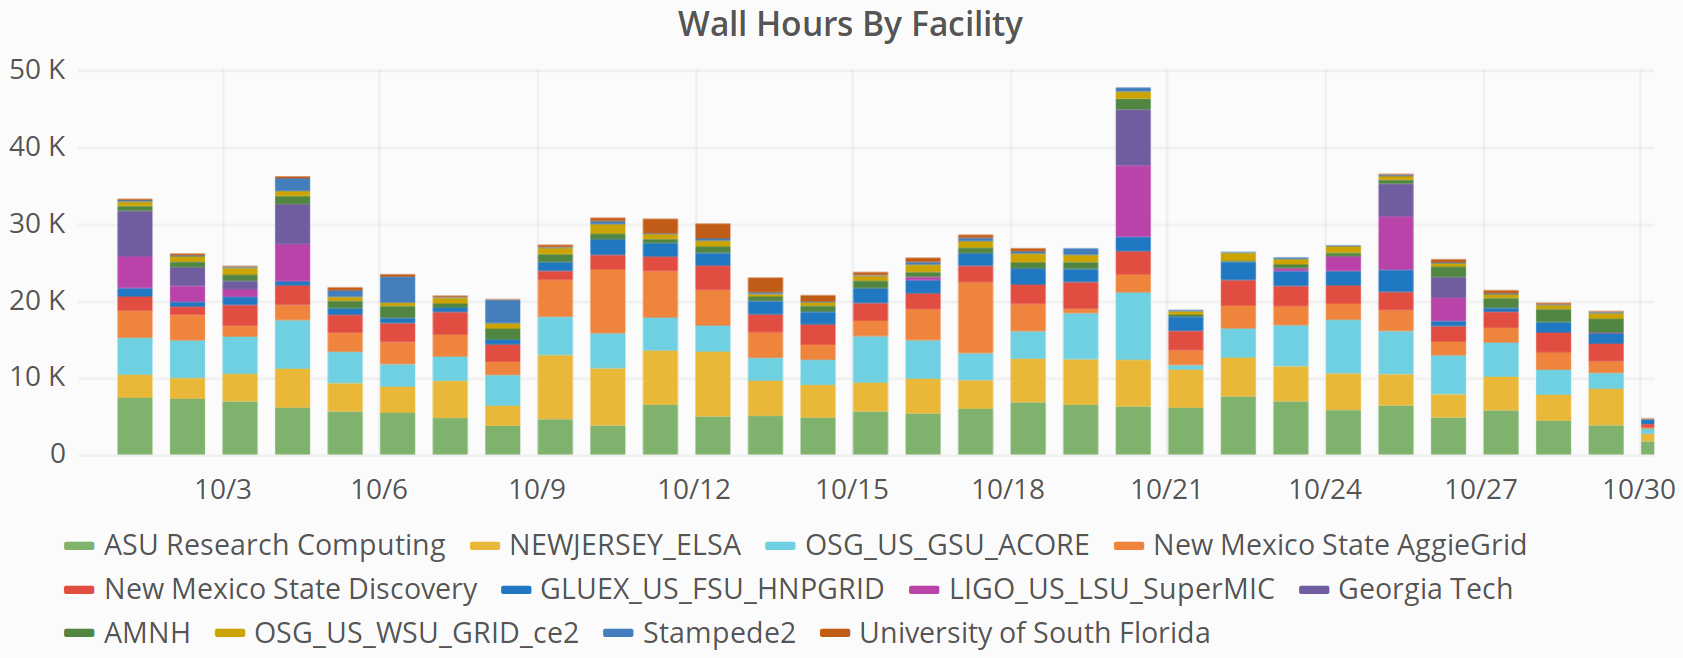
\includegraphics[width=1.0\textwidth]{images/WallByFacility.png}
\caption{A subset of facilities that are using the Hosted CE initiative to share their resources}
\label{fig-WallByFacility}
\end{figure}

\section{Conclusions}
\label{conclusions}
With the Hosted CE initiative, the hardware/software stack needed to operate a CE is maintained by OSG Operations staff in a homogeneous and automated way. This provides a reduction in the overall operational effort needed to maintain the CEs: one single organization does it in an uniform way, instead of each single resource provider doing it in their own way.

Currently, more than 20 institutions are exploiting the Hosted CE initiative to make their resources available to different scientific communities. This means that 20 different site administrators did not have to learn how to install a Compute Element, and their institution did not have to provide the required hardware for running the service as well as guaranteeing operational coverage for the CE in the future. Instead, OSG takes care of everything and it is able to do it in a semi-automated way, while also taking care of communication with site administrators in case of issues.

A solution that uses containers is being explored to further reduce the operational footprint needed to maintain the CEs. In this way the hardware requirements to run the CEs will be reduced (containers are lighter than virtual machines), and installing a CE is going to be even easier and more streamlined.

\section*{Acknowledgements}
\label{acknowledgements}

\begin{acknowledgement}
This material is based upon work supported by the National Science Foundation under Grant
No. NSF MPS-1148698
\end{acknowledgement}

\bibliography{papers}

\end{document} 